\documentclass[../../Main/Main.tex]{subfiles}

\begin{document}


\chapter{Non ideal fluids: Mean field theory, Van der Walls, Virial expansion and Cluster expansion}

\section{Mean field theory for fluids}

Ideal gases are exceedingly idealised systems and are not suited to describe the behaviour of real systems: they always obey the same state equation and never undergo phase transitions (for example they never condense). We must therefore step a little further: using the "philosophy" of mean field theories we can make the description of fluids a little bit more realistic. As we will see this will also lead to the derivation of the Van der Waals equation, which better describes the behaviour of real fluids (even if, as we will shortly see, it still has some problems).

In general, in a real gas all the atoms or molecules interact through a certain potential \(\Phi(\{\va{r}_i\})\) that will depend on the positions of all the particles. For a fluid system of  \( N \) particles  with position vectors \( \{ \va{r}_i \}_{i=1,\dots,N}   \), the configurational contribution to the (grancanonical) partition function will therefore be:

\begin{equation}
  Q_N (T) = \int_{V}^{} \prod_{i=1}^{N}  \dd[]{\va{r}_i}  e^ {-\beta  \qty( \Phi(\{\va{r}_i\}) + \sum_{i=1}^{N} \psi _{ext}  (\va{r}_i) ) }
\end{equation}
where \( \psi _{ext} \) is a one body external potential, but we do not consider it because is not the aim of our problem. In general,
\begin{equation*}
  \Phi (\{ \va{r}_i \}  ) = \sum_{i\neq j}^{}  U_2 (\va{r}_i,\va{r}_j) + \sum_{i\neq j\neq \mu }^{} U_3 (\va{r}_i, \va{r}_j, \va{r}_ \mu ) + \dots
\end{equation*}
(where \(U_{n} \) can be a generic \(n\)-body interaction potential). For simplicity, we do not consider \( U_3 \), that is the three body interaction. Let us suppose
\begin{equation*}
   U_2 (\va{r}_i,\va{r}_j) \rightarrow U_2 ( \abs{\va{r}_i - \va{r}_j} )
\end{equation*}
Therefore,
\begin{equation*}
  Q_N (T) = \int_{V}^{} \prod_{i=1}^{N}  \dd[]{\va{r}_i}  e^ {-\beta \sum_{i\neq j }^{}  U_2 ( \abs{\va{r}_i - \va{r}_j} ) }
\end{equation*}
Now, we replace all this story with just a field, it is a sort of average of the interactions. Doing the mean field assumption for \( U_2 \), we obtain
\begin{equation*}
  \sum_{i,j > 1 }^{}  U_2 ( \abs{\va{r}_i - \va{r}_j} ) \rightarrow \sum_{i}^{} \Phi _{MF} (\va{r}_i)
\end{equation*}

Generally \(\psi _{ext}\) does not pose great problems while it is \(\Phi\) that makes \( Q_{N}\) impossible to compute exactly, forcing us to resort to approximations. In the framework of mean field theories, we substitute the interaction potential \(\Phi\) with an effective single-particle potential  that acts on every particle in the same way. Hence,  the \textit{mean field approximation}  consists in substituting the multi-body interaction potential \(   \Phi (\{ \va{r}_i \}  ) \) with an effective one body potential \( \Phi (\va{r}) \) withing which all the particles move:
\begin{empheq}[box=\myyellowbox]{equation}
\Phi (\{ \va{r}_i \})   =\sum_{i}^{} \Phi _{MF} (\va{r}_i)
\end{empheq}
As said, for simplicity consider \( \psi _{ext} = 0 \), hence mean field theories allow us to compute \(Q_N\) as
\begin{equation}
  Q_N^{MF} (T) \simeq \qty[  \int_{V}^{}  \dd[D]{\va{r}}  e^ {-\beta \Phi _{MF} (\va{r})  } ]^N
\end{equation}

\begin{remark}
The integral depends on the form of \( \Phi _{MF} (\va{r})  \). Of course, every particular mean field theory will provide a different form of \( \Phi _{MF} (\va{r})  \) which will lead to different results.
\end{remark}

If one assumes \emph{spatial isotropy},
what it is important is not anymore the vector but only the distance; hence, it is important just the integral over the modulus:
\begin{equation*}
    \Phi _{MF} (\va{r}) = \Phi _{MF} (\abs{\va{r}} ) = \Phi _{MF} (r)
\end{equation*}

\section{Van der Waals equation}
The Van der Waals equation can be obtained considering the atoms of a gas as hard spheres. In this case, in fact, the mean field has the form:
\begin{equation}
\Phi _{MF} (r) =
  \begin{cases}
   \infty & r < r_0 \quad  \text{repulsion}\\
   u < 0 & r> r_0  \quad \text{attraction}
  \end{cases}
\end{equation}
as plotted in Figure \ref{fig:14_1}.
\begin{figure}[H]
\centering
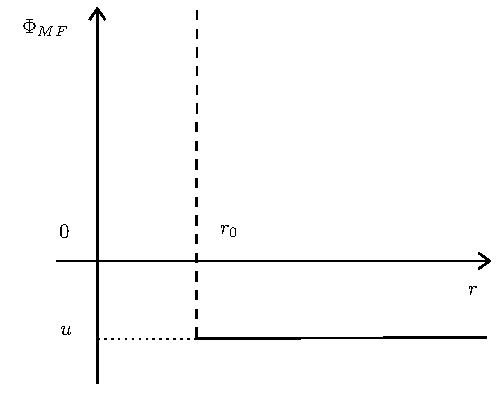
\includegraphics[width=0.6\textwidth]{./img/1.pdf}
\caption{\label{fig:14_1} Plot of the potential \( \Phi _{MF} (r) \).}
\end{figure}


\noindent The partition function becomes
\begin{equation*}
  Q_N^{MF} (T) = \qty[ V_{ex}e^{- \infty } + (V-V_{ex})e^{-\beta u} ]^N
\end{equation*}
where \( V_{ex} \simeq r_0^3 \) is the volume not accessible by the particle. Finally, the result is
\begin{equation}
  Q_N^{MF} (T) = \qty[ (V-V_{ex})e^{-\beta u} ]^N
\end{equation}
The free energy is \( F_N = -k_B T \ln Q_N \), hence
\begin{empheq}[box=\myyellowbox]{equation}
  F_N^{MF} (T) = - N k_B T \qty[ \ln{(V-V_{ex})} - \beta u ]
\end{empheq}
Let us calculate the pressure
\begin{equation}
  P_N^{MF} = - \eval{\pdv{F_N^{MF}}{V} }_T = \frac{N k_B T}{V-V_{ex}} - N \qty(\pdv{u}{V} )_T
  \label{eq:14_1}
\end{equation}
\begin{remark}
In general, the deep \( u \)  can go up and down depending on the \emph{V}: \( u = u (V) \). This is because \( u \) is the attractive well of the mean field potential and, for \( r \ge r_0 \) must be proportional to the fluid density
\begin{equation*}
  u \sim -N/V
\end{equation*}
where the minus sign means attraction. On the other hand, also \( V_{ex} \), the volume not accessible, must be proportional to \( N \).
\end{remark}
Hence, we have
\begin{equation*}
  u = - a \frac{N}{V}, \qquad V_{ex} = b N
\end{equation*}
where \( b \) is the volume of a single particle.
Inserting the last term in \eqref{eq:14_1}, we obtain the \emph{Van der Walls equation of state}:
\begin{empheq}[box=\myyellowbox]{equation}
  P_N^{MF} (V,T) = \frac{N k_B T}{V-bN} - a \qty(\frac{N}{V})^2
  \label{eq:14_2}
\end{empheq}



\subsection{Critical point of Van der Waals equation of state}
Let us define the specific volume as
\begin{equation*}
  v \equiv \frac{1}{\rho } = \frac{V}{N}
\end{equation*}
Hence, the equation of state becomes
\begin{equation}
P = \frac{K_B T}{v - b} - \frac{a}{v^2}
\end{equation}

The behaviour of the Van der Waals isotherms is shown in Figure \ref{fig:14_2_1}. As we can see this changes with the temperature and resembles that of real isotherms; however, Van der Waals isotherms are always analytic and have a non physical behaviour in certain regions of \( (v,P)\) plane, called spinodal curves, if \( T < T_c\): for some values of \(v\) we have \( \partial P / \partial v >0\) which is physically impossible. This is a consequence of the roughness of the approximation we have made, since it can be shown that it doesn't ensure that the equilibrium state of the system globally minimizes the Gibbs free energy. As we will shortly see, however, this problem can be solved "by hand" with Maxwell's equal area rule, or Maxwell's Construction. Overall, we have this effect because it is a mean field, so the curve in Figure \ref{fig:14_2_1} it is replaced by the curve in Figure \ref{fig:14_2_2}.
Moreover, for \( T < T_c \) the equation \( P(v) = const \) has 3 distinct solutions. For \( T > T_c \) only one solution \( \in \R \).


\begin{figure}[H]
\begin{minipage}[c]{0.5\linewidth}
\subfloat[][ Van der Waals isotherms are represented in red in \( (v,P) \) diagram for different values of \(T\). ]{ 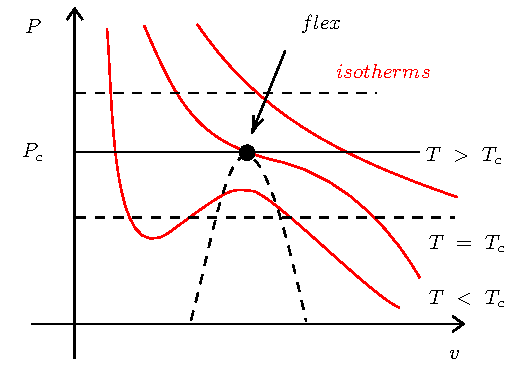
\includegraphics[width=0.9\textwidth]{./img/2.pdf}  \label{fig:14_2_1} }
\end{minipage}
\begin{minipage}[]{0.5\linewidth}
\centering
\subfloat[][Real isotherm in \( (v,P)\) diagram for \(T<T_c\). ]{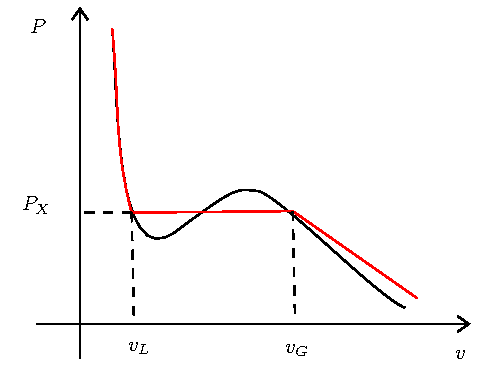
\includegraphics[width=0.9\textwidth]{./img/3.pdf}  \label{fig:14_2_2} }
\end{minipage}
\caption{\label{fig:} }
\end{figure}

Let us now see how to determine the critical point of a system obeying Van der Waals equation.

\begin{itemize}
\item First of all, from the representation of the isotherms we can see that the critical point is a flex for the critical isotherm (i.e. the one with \(T=T_c\)); in other words, we can determine the critical point from the equations:
\begin{equation*}
  \pdv{P}{v} = 0, \qquad \pdv[2]{P}{v} = 0
\end{equation*}
 The second in particular means that there is a flex point. Let us pay attention to it, indeed it is a standard way to find critical points.
We obtain
\begin{equation*}
  v_c = 3 b, \quad  P_c = \frac{a}{27 b^2}, \quad k_B T_c = \frac{8a}{27b}
\end{equation*}


\item Another way to find the critical point consists in noticing that at \( T=T_c \), the 3 solutions coincide. In fact, we can note that the equation \(P (v)= P = const \) is cubic in \(v\). Let us rewrite the Van der Waals equation
\begin{equation*}
  P = \frac{v^2 k_B T - a (v-b)}{v^2 (v-b)}
\end{equation*}
as
\begin{equation}
  v^3 - \qty(b + \frac{k_B T}{P})v^2 + \frac{a}{P} v - \frac{a b }{P} = 0
  \label{eq:14_3}
\end{equation}
For \(T>T_c\) this equation has one real solution and two imaginary ones, and for \(T<T_c\)  three distinct real solutions; when \(T=T_c\) the three solutions of the equation coincide. This means that at the critical point \( T=T_c \) this last equation Eq.\eqref{eq:14_3}  must be written in the form:
\begin{equation*}
  (v-v_c)^3 = 0 \quad \Rightarrow v^3 - 3 v^2 v_c + 3 v v_c^2 - v_c^3 = 0
\end{equation*}
Equating the coefficients with Eq.\eqref{eq:14_3} we get:
\begin{equation*}
  v_c^3 = \frac{a b}{P_c}, \quad 3 v_c^2 = \frac{a}{P_c}, \quad 3 v_c = b + \frac{k_B T_c}{P_c}
\end{equation*}
from which we have again:
\begin{equation}
  v_c = 3 b, \quad P_c = \frac{a}{27 b^2}, \quad k_B T_c = \frac{8 a }{27 b }
  \label{eq:14_4}
\end{equation}
We have found a very interesting result: in fact, if we can measure \(a\) and \(b\) at high temperatures then we are able to determine the critical point of the system.

This model has also an interesting property, since it predicts that:
\begin{equation*}
    \frac{P_c v_c}{k_B T_c} = \frac{3}{8}  \approx 0.375
\end{equation*}
which is a universal number, independent of \(a\) and \(b\) and so of the particular fluid considered. Experimentally this ratio is approximately 0.29 for Argon, 0.23 for water and 0.31 for  \( \text{He}^4 \).
Therefore, even if it is very rough, this model leads to reasonable conclusions.

\end{itemize}



\subsection{Law of corresponding states}
The universal value of the ratio \( \frac{P_c v_c}{k_B T_c} \) suggests a deeper correspondence between different fluid systems.
We can also rewrite Van der Waals equation \eqref{eq:14_2} in a dimensionless form, rescaling the thermodynamic quantities of the system. In particular, defining:
\begin{equation}
  \pi \equiv \frac{P}{P_c}= P\frac{27b^2}{a}, \quad \nu  \equiv \frac{v}{v_c} = \frac{v}{3b}, \quad \tau \equiv \frac{T}{T_c} = k_B T\frac{27b}{8a}
\end{equation}
Van der Waals equation becomes:
\begin{empheq}[box=\myyellowbox]{equation}
  \qty(\pi + \frac{3}{\nu ^2}) \qty(3 \nu -1) = 8 \tau
\end{empheq}
We have found another very interesting result: when rescaled by their critical thermodynamic properties (by \( P_c, v_c \) and \( T_c \)), all fluids obey the same state equation. This is the law of corresponding states: this is a form of universality. The law of corresponding states applies everywhere on the phase diagram. It can even be shown that this law is a consequence of dimensional analysis, and is more general than what might seem: experimentally the law of corresponding states is well satisfied also by fluids which do not obey Van der Waals equation.



\subsection{Region of coexistence and Maxwell's equal area rule}
In real fluids, for \( T < T_c \) \( (\tau < 1) \), there is a first order liquid-gas transition with coexistence between vapor and liquid phase and non analiticity of the thermodynamic potential. In particular, a real isotherm for \( T < T_c \) is the one in Figure \ref{fig:14_2_2}. How this is described by the mean-field (i.e. Van der Walls) theory?
The Van der Walls isotherm for \(T<T_c\) is given by the graphic in Figure \ref{fig:14_3}.
\begin{figure}[H]
\centering
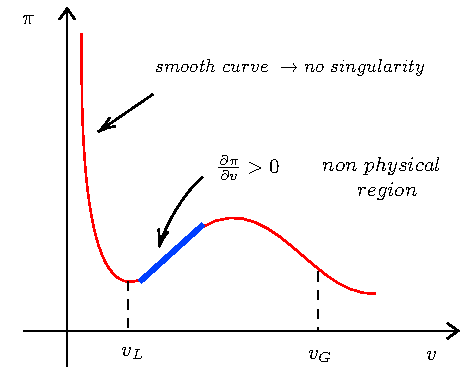
\includegraphics[width=0.7\textwidth]{./img/4.pdf}
\caption{\label{fig:14_3} Van der Waals isotherm for \(T<T_c\).}
\end{figure}
The liquid phase goes into a phase region that is not thermodinamycally stable.
How can we remove the non physical regions of the Van der Walls equation of state and describe coexistence? The solution is the Maxwell (or equal area) construction!


\subsubsection{Equal area or Maxwell construction}
As we have previously anticipated, Maxwell's equal area rule is a method to "manually" remove the unphysical regions of Van der Waals isotherms.

From phase coexistence and general properties of phase transitions we know that at the coexistence of two phases the chemical potentials and the pressures of the two phases must be equal;  furthermore, from thermodynamic potentials we also know that the chemical potential is the Gibbs free energy per particle, namely \(G=\mu N \), and in general we have also:
\begin{equation*}
    \dd[]{G} = - S \dd[]{T} + V \dd[]{P} + \mu \dd[]{N}
\end{equation*}
Now, differentiating \(G=\mu N\) and subtracting this last equation we get:
\begin{equation*}
  \dd[]{\mu } = - \frac{S}{N} \dd[]{T} + \frac{V}{N} \dd[]{P}
\end{equation*}
Therefore, since along an isotherm  \( \dd[]{T}=0\), we will have:
\begin{equation*}
  \dd[]{\mu } = \frac{V}{N} \dd[]{P}
\end{equation*}
At the coexistence we have also \( \dd[]{P}_{coex}= 0  \), hence
\begin{equation*}
  \dd[]{\mu } = 0
\end{equation*}
is the physical condition.
Recall that for Van der Wall \( \dd[]{P} \neq 0  \)!
Hence, the physical coexistence condition implies
\begin{equation*}
  0 = \int_{1}^{2} \dd[]{\mu } = \mu (2) - \mu (1) \overset{Van\, der\, Walls}{=} \frac{1}{N} \int_{P_G}^{P_L} \dd[]{P} V
\end{equation*}
\begin{figure}[H]
\centering
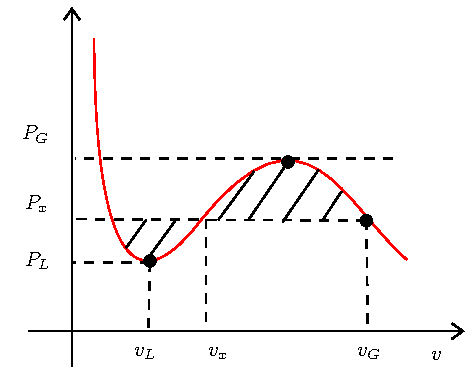
\includegraphics[width=0.6\textwidth]{./img/5.pdf}
\caption{\label{fig:14_4} Maxwell's equal area rule: Van der Walls isotherm for \( T < T_c \).}
\end{figure}
Looking also at the Figure \ref{fig:14_4}, we see that this means that the horizontal segment of the isotherm must be drawn so that the two regions have the same area (from which the name of the method).
The integral can be partitioned in two parts
\begin{equation*}
  0 = \int_{P_G}^{P_L} V \dd[]{P} \quad \Rightarrow \int_{P_G}^{P_x} V\dd[]{P} = - \int_{P_x}^{P_L} \dd[]{P} V
\end{equation*}
Hence, the equal area condition gives the value of \( P_x \) of the coexistence line!


\clearpage


\subsection{Critical exponents of Van der Walls equation}
Let us now study the behaviour of systems obeying Van der Waals equations near the critical point, computing one of the critical exponents.

\subsubsection{\( \pmb{\beta}  \) exponent}
The equation of state for Van der Walls is:
$$\left( \pi + \frac{3}{v^{2}} \right)(3\nu-1)= 8\tau$$

where
$$\pi = \frac{P}{P_{c}}, \nu = \frac{v}{v_{c}},\tau = \frac{T}{T_{c}}$$
We know that for $T < T_{c}$ ($\tau <1$) the Van der Walls equation of state has 2 stable solutions $\pi_{g} = \pi_{l}$:
$$\pi = \frac{8\tau}{3\nu_{l} - 1} - \frac{3}{\nu_{L}^{2}} = \frac{8\tau}{3v_{G}-1} - \frac{3}{v_{G}^{2}}$$
where $\nu_{L} = \nu_{Liquid}, \nu_{G}=\nu_{Gas}$.
Solving for $\tau$ gives:

$$\tau = \frac{(3\nu_{L}-1)(3\nu_{G} - 1)(\nu_{L} + \nu_{G})}{8\nu_{G}^{2}\nu_{L}^{2}}$$
As we approach $T_{c}$ we have $\nu_{G}, \nu_{L} \to 1$ by definition of $\nu$ and we get $\tau \to 1$, as expected.
Let us expand the right hand side for small $\delta = \nu_{G} - \nu_{L}$.
The equation for $\tau$ being symmetric in $\nu_{G},\nu_{L}$ we can write 
$$\nu_{G} = 1 + \frac{\delta}{2}, \nu_{L} = 1 - \frac{\delta}{2}$$
By substituting in we get
$$
\begin{aligned}
& \tau \sim \frac{(3(1-\delta / 2)-1)(3(1+\delta / 2)-1) \cdot 2}{\delta(1+\delta / 2)^2(1-\delta / 2)^2} \\
& \sim \frac{\left(2-\frac{3}{2} \delta\right)\left(2+\frac{3}{2} \delta\right)}{4(1+\delta)(1-\delta)} \sim \frac{\left(1-\frac{3}{4} \delta\right)\left(1+\frac{3}{4} \delta\right)}{1-\delta^2} \\
& \sim \frac{1-\frac{9}{16} \delta^2}{1-\delta^2} \sim1-\frac{9}{16} \delta^2 \sim 1-\frac{9}{16}\left(v_g-v_e\right)^2 \\
& \Rightarrow \tau \sim 1-\frac{9}{16}\left(v_g-v_e\right)^2 \quad \tau=\frac{T}{T_c} \\
& \Leftrightarrow - \left( \frac{T}{T_{c}} - 1 \right) \sim \frac{9}{16}(v_{G} - v_{L})^{2 }\\
& \Rightarrow v_g-v_e \stackrel{T \rightarrow T_c}{\sim}\left(\frac{T_c-T}{T_c}\right)^{1 / 2}
\end{aligned}
$$

Hence
$$
\boxed{ \beta=\frac{1}{2} }
$$




\subsubsection*{Delta Exponent}

From the Van der Walls equation of state we know that, at $T = T_c$ , for a given volume $v_{c}$, there is a unique solution $p_{c}$. On the other hand at the critical point we know that
$$\frac{ \partial P }{ \partial v  }\bigg\rvert_{v_{c}} = \frac{ \partial ^2 P }{ \partial v ^{2} }\bigg\rvert_{v_{c}} = 0 $$
So if we expand $p$ in proximity of $p_{c}$ around $v = v_{c}$ we know that the first two derivatives are zero so by taylor expansion around $p_{c}$ we get
$$P \approx p_{c} + (v- v_{c})^{3}\frac{ \partial^{3} P }{ \partial v^{3}  }\bigg\rvert_{v_{c}} + \dots $$
So
$$p - p_{c} \approx (v-v_{c})^{3} \implies \boxed{ \delta = 3 }$$
Experiments on gases close to their critical points gives 
$$(v_{G} - V_{L}) \sim (T_{c} - T)^{\beta}, \beta \approx 0.32$$
$$p - p_{c} \sim (v - v_{c})^{\delta}, \delta = 4.8$$

\textbf{So the estimates of the critical exponents based on the Van der Walls (mean field) theory are not very accurate!}


\section{Theories of weakly interacting fluids}
If the gas is not ideal but made by weakly interacting particles, it is possible to follow a \emph{perturbative approach}  to compute the partition function of such systems. Let us consider \( N \) particles in region \( \Omega  \) of volume \( V \). Particles interact through a generic two-body potential that depends only on the relative distance between the particles:
\begin{equation*}
  U_2 ( \va{r}_i, \va{r}_j) = \Phi (\abs{\va{r}_i - \va{r}_j} )
\end{equation*}
Hence,
\begin{equation}
  \Rightarrow U ( \{ \va{r} \}  ) = \frac{1}{2} \sum_{i,j}^{} \Phi (\abs{\va{r}_i - \va{r}_j} )
\end{equation}
The Hamiltonian then is:
\begin{equation}
  \mathcal{H}_ \Omega (\{ \va{r} \}  ) = \sum_{i=1}^{N} \frac{\va{p}_i^2}{2m} + \sum_{i,j>i}^{} \Phi (\abs{\va{r}_i - \va{r}_j} )
\end{equation}
and its partition function in the canonical ensamble:
\begin{equation}
  Z_ \Omega (N,V,T) = \frac{1}{N! \Lambda ^{3N}} Q_N (V,T)
\end{equation}
where
\begin{equation}
  Q_N (V,T) = \int_{V}^{} \dd[]{\va{r}_1} \int_{V}^{} \dd[]{\va{r}_2} \dots \int_{V}^{} \dd[]{\va{r}_N} \exp [- \beta U (\{ \va{r} \}  )]
\end{equation}
\begin{remark}
Of course for ideal gases \( U = 0 \), and so
\begin{equation*}
  Q_N (V,T) = V^N \quad \rightarrow Z_N^{ideal} = \frac{V^N}{N! \Lambda ^{3N}}
\end{equation*}
and the dependence on \( T \) is exclusively due to \( \Lambda = \Lambda (T) \) (i.e. kinetic energy).
\end{remark}
Now, suppose \( U \neq 0 \), but small!
If we consider also the interaction terms we must insert a correction \( \chi  \) in the configurational contribution to the partition function.
 We can say that our \( Q_N (V,T) \) it would be the on of the ideal version times a new function
\begin{equation}
 Q_N (V,T) \simeq V^N \chi (N,V,T)
\end{equation}
which depending on the possible presence of attractive terms in the interaction potential \( \Phi  \) can in general be also a function of the temperature \( T \);
furthermore the correction depends strongly on the gas density: if it is low the particles will not "perceive" the presence of the other ones and the ideal gas approximation is a good one, while for high densities the particles will be closer to each other and corrections to \( Q_N \) are necessary.
\begin{remark}
If \( \Phi  \) is only repulsive, \( \chi  \) does not depend on \( T \).
\end{remark}
Let us note that inserting the correction \( \chi  \), the free energy of the system will be:
\begin{equation}
  F_N = F_N^{ideal} - k_B T \ln{\chi }
\end{equation}
As previously said, the correction \( \chi  \) due to particle-particle interaction depends on the particle density \( \rho  \) of the fluid:
\begin{equation}
  \begin{cases}
   \rho _{small} &\Rightarrow  U = 0 \\
   \rho _{high} &\Rightarrow  U \neq 0 \text{ and not negligible}
  \end{cases}
\end{equation}
This suggests that the equation of state of a weakly interacting gas can be expanded formally in powers of \( \rho  \). This is known as \emph{virial expansion}.

In particular, for the ideal gas:
\begin{equation*}
  \frac{P}{k_B T} = \rho
\end{equation*}
For a non ideal gas, let us add the other terms of the expansion
\begin{equation}
  \rightarrow \frac{P}{k_B T} = \rho + B_2 (T) \rho ^2 + B_3 (T)\rho ^3+ \dots + O(\rho ^n)
  \label{eq:14_6}
\end{equation}
this is a virial expansion and it is one of the most used. The coefficient \( B \) are called the \emph{virial coefficients}.
The Eq.\eqref{eq:14_6} was first introduced as a formula to fit experimental data. Indeed, making a fit, you will obtain the virial coefficients. This is what physicist have done for years.  Then, mapping the coefficient with the real world experiments, we can find some macroscopical parameters.
The formula \eqref{eq:14_6} can be also obtained rigorously from a perturbation approach to the partition function (as we will see later). Now, the question is: which is the virial expansion of a Van der Walls (i.e. mean field) gas?


\subsection{Van der Walls and virial expansion}
Let us see for example the virial expansion of the Van der Waals equation. From Van der Waals equation we have:
\begin{equation*}
  \frac{P}{k_B T} = \frac{N}{V-bN} - \frac{a N^2}{k_B T V^2}
\end{equation*}
Let us factorize the term \( (N/V) \),
\begin{equation*}
  \frac{P}{k_B T} = \qty(\frac{N}{V}) \qty(1 - b \frac{N}{V})^{-1} - \frac{a}{k_B T}\qty(\frac{N}{V})^2
\end{equation*}
Then, by expanding in power of \( (N/V) \) and defining \( \rho = N/V \), we have
\begin{equation*}
\begin{split}
  \Rightarrow \frac{P}{k_B T}  &= \qty(\frac{N}{V}) + \qty(\frac{N}{V})^2 \qty(b - \frac{a}{k_B T}) + \qty(\frac{N}{V})^3 b^2 + \qty(\frac{N}{V})^4 b^3 + \dots \\
  & = \rho + \qty(b - \frac{a}{k_B T})\rho ^2 + b^2 \rho ^3 + b^3 \rho ^4 + \dots
\end{split}
\end{equation*}
We can thus immediately identify the first virial coefficient:
\begin{equation*}
  B_2 (T)^{VdW} = b - \frac{a}{k_B T}, \qquad B_3^{VdW} = b^2
\end{equation*}
where in \( B_2 (T)^{VdW}  \) the first term is repulsive on excluded volume and the second one is the attraction term. We note also that \( B_3^{VdW} \) is always positive.

\subsubsection{Boyle's temperature \( T_B \) }
The Boyle's temperature is the \( T \) at which the second coefficient is zero:
\begin{equation*}
  B_2^{VdW} (T_B) = 0
\end{equation*}
so we have removed the most important coefficient. The competiting effects of repulsion and attraction are cancelled out. In this case, the Van der Walls temperature \( T_B^{VdW} \) is
\begin{equation*}
  T_B^{VdW} = \frac{a}{b k_B}
\end{equation*}
to be compared with the critical temperature \( T_c^{VdW} \) that is
\begin{equation*}
  T_c^{VdW} = \frac{8 a}{27 b^3 k_b}
\end{equation*}
We notice that \( T_c^{VdW} \ll T_B ^{VdW} \).  It is clear that the Boyle's temperature must be much greater than the critical one.

\begin{remark}
   Consider a polymer, the transition point called the \( \theta  \) point is when the second coefficient is zero, as the case described above, but it is interesting in polymer kind of system (lesson).
\end{remark}

\subsection{Cluster expansion technique for weakly interacting gases}

We now obtain the formal virial expansion by starting from the microscopic system and performing a perturbation expansion of the Boltzmann weights for small values of \( U \).
Let us start from the partition function
\begin{equation}
  Q_N = \int_{V}^{} \dd[]{\va{r}_1} \dots \int_{V}^{} \dd[]{\va{r}_N}  e^{-\beta U (\{ \va{r} \}  ) } = \int_{V}^{} \dd[]{\va{r}_1} \dots \int_{V}^{} \dd[]{\va{r}_N}  e^{-\beta \sum_{i,j > i}^{} \Phi _{ij} }
\end{equation}
where we have used the short notation
\begin{equation*}
  \Phi _{ij} \equiv \Phi (\abs{\va{r}_i - \va{r}_j} )
\end{equation*}
The idea is to find a "small quantity" in terms of which we can expand \( Q_N \); this quantity is the so called \emph{Mayer function}.
\begin{definition}{Mayer function}{}
  The \emph{Mayer f-function} is an auxiliary function that often appears in the series expansion of thermodynamic quantities related to classical many-particle systems. It is defined as
  \begin{equation}
    f (\abs{\va{r}} ) \equiv e^ { - \beta \Phi ( \abs{\va{r}} )} -1
  \end{equation}
  \begin{remark}
  Note: if \( \beta \Phi (r) \ll 1 \), we have \( f(r) \ll 1 \).
  \end{remark}
\end{definition}
In fact, when the gas is ideal  \( f(\va{r}) = 0 \), and if the particles interact weakly \( \Phi  \) is small, and so is \( f(\va{r})  \).
In particular, this expansion will work well for low densities (namely \( | \va {r}_i - \va{r}_j| \)  is large and so \( \Phi  (|\va {r}_i - \va{r}_j| ) \to 0 \)) or high temperatures (namely \( \beta \to 0  \)): in both cases, in fact, \( e^{-\beta  \Phi  (|\va {r}_i - \va{r}_j| )} \rightarrow 1 \) and \( f  (|\va {r}_i - \va{r}_j| ) \to 0 \).
 Using the short notations \(   \Phi _{ij} \equiv \Phi (\abs{\va{r}_i - \va{r}_j} ) \) and \( f_{ij} \equiv f (\abs{\va{r}_i - \va{r}_j} ) \) we have
\begin{equation*}
\begin{split}
  \Rightarrow e^{-\beta \sum_{i}^{}  \sum_{j>i}^{} \Phi _{ij}  } &= \prod_{i}^{} \qty(\prod_{j>i}^{} (1+ f_{ij})  ) \\
  & = \underbrace{(1+f_{12})(1+f_{13})  \dots ( 1 + f_{1N })}_{i=1}   \dots \underbrace{(1+f_{23}) (1+ f_{24}) \dots ( 1 + f_{2N })}_{i=2} \dots \\
  & = (1 + f_{12} + f_{13} + f_{12}f_{13}) (1+f_{14}) \dots(1+f_{23}) \\
  & = 1 + \sum_{i}^{} \sum_{j>i}^{} f_{ij} + \cancel{\sum_{i=1}^{N} \sum_{k \ge i}^{} \sum_{l > k}^{} \sum_{j > i }^{} \sum_{(ij) \neq (lk)}^{}  f_{ij} f_{kl}       } + O (f^3)
\end{split}
\end{equation*}
where
\begin{equation*}
  f_{ij} \equiv  e^{-\beta \Phi _{ij}} -1
\end{equation*}
Higher order terms contain products of \( 3,4,\dots f_{ij} \) terms. For simplicity, let us consider first only linear terms. Hence, the solution is given by considering only the linear term. This is the cluster expansion.


As said, this first approximation is reasonable if either
\begin{enumerate}
\item \( \rho  \) is small enough. It implies that \( \abs{\va{r}_i - \va{r}_j} \gg 1 \) and hence \( \Phi _{ij} \ll 1 \).
\item Sufficiently high \( T \) such that \( \Phi (\abs{\va{r}_i - \va{r}_j} )/k_B T \ll 1 \). What is important it is the ration between \( \beta  \)  and \( \Phi _{ij} \).
\end{enumerate}
In either cases we have \( \exp (- \beta \Phi _{ij}) \rightarrow 1 \) and \( f_{ij} \rightarrow 0 \). By keeping only linear terms,  the configurational contribution to the partition function will be
\begin{equation*}
\begin{split}
  Q_N (V,T) &= \int_{V}^{} \dd[]{\va{r}_1} \dots \dd[]{\va{r}_N} \qty(1+ \sum_{i,j>i}^{} f_{ij} + \dots )
  = V^N + \sum_{i,j>i}^{} \int_{V}^{} \dd[]{\va{r}_1} \dots \int_{V}^{}  \dd[]{\va{r}_N} f_{ij} \\
  &= V^N + V^{N-2} \sum_{i,j>i}^{} \int_{V}^{} \dd[]{\va{r}_i} \dd[]{\va{r}_j} f_{ij} + \dots \\
\end{split}
\end{equation*}
We are summing up over all configurations \( ij \). Let us try to compute the double integral, with the definition of a new variable \( \va{r} = \va{r}_i - \va{r}_j \):
\begin{equation*}
  \int_{V}^{} \dd[]{\va{r}_i} \int_{V}^{} \dd[]{\va{r}_j} f_{ij} (\abs{\va{r}_i - \va{r}_j} ) \underset{\substack{ \text{translational} \\  \text{symmetry} } }{=}  \int_{V}^{} \dd[]{\va{r}_i} \int_{V}^{}  \dd[]{\va{r}} f (\va{r})
  = V \int_{V}^{} \dd[]{\va{r}}  f \qty(\abs{\va{r}} ) \equiv -2 B_2 V
\end{equation*}
Hence,
\begin{equation}
  B_2 \equiv - \frac{1}{2} \int_{V}^{} \dd[]{\va{r}}  f \qty(\abs{\va{r}} )
\end{equation}
From this we see precisely how the virial coefficient, which as we have already stated can be experimentally measured, is related to the microscopic properties of the interaction between the particles, represented by the Mayer function \( f \). It can also be shown that all the virial coefficients can be expressed in terms of integrals of products of Mayer functions: higher order coefficients involve the computation of increasingly difficult integrals, which can however be visualized in terms of graphs.

What we have seen now is how the cluster expansion works in general. Let us now apply it in order to find the virial expansion for real gases. From what we have found, the configurational partition function of the system becomes:
\begin{equation*}
  Q_N (V,T) = V^N -  V^{N-1} 2 B_2 (T)  \sum_{i,j>i}^{} 1 + \dots
\end{equation*}
The remaining sum is equal to \( N(N-1)/2 \): in fact, for any of the \( N \) values that
\( i \) can assume,  \( j \)  can have \( N-1 \) values. These are all the possible connections (bonds) between pairs of particles \( (i,j) \) with \( j>i \).
Hence,
\begin{equation}
  Q_N (V,T) = V^N - V^{N-1}  B_2 (T)  N (N-1) + \dots
\end{equation}
and, considering that  \( N-1 \approx N \) for large \( N \), the complete partition function of the system will be:
\begin{equation}
  Z_N (V,T) = \qty(\frac{V^N}{N! \Lambda ^{3N}}) \qty(1- \frac{N^2}{V} B_2 (T)+ \dots)
\end{equation}
We recognise in this expression that \( (1-B_{2}N^{2}/V+\cdots ) \) is the correction \( \chi  \) to the ideal gas partition function that we have mentioned earlier; therefore, the free energy of the system will be:
\begin{equation}
  F_N = F_N^{ideal} - k_B T \ln{\qty[1-\frac{N^2}{V}B_2 (T)+ \dots] }
\end{equation}
and its pressure:
\begin{equation*}
  P_N = - \qty(\pdv{F_N}{V} )_{T,N} = \frac{N k_B T}{V} \qty(1+ \frac{\frac{N}{V}B_2}{1- \frac{N^2}{V}B_2})
  = \frac{N k_B T}{V} \qty(\frac{1 -\frac{N^2}{V} B_2 + \frac{N}{V} B_2 }{1- \frac{N^2}{V} B_2})
\end{equation*}
Expanding the denominator for \( \frac{N}{V} B_2 \ll 1 \) so \( \rho \ll 1 \), one gets
\begin{empheq}[box=\myyellowbox]{equation}
  P_N \simeq \frac{N k_B T}{V} \qty(1+\frac{N}{V}B_2 + \dots)
  \label{eq:15_1}
\end{empheq}
here we see the correction to the ideal gas.
\begin{remark}
The equation \eqref{eq:15_1} gives an important relation between experimentally accessible observables as \( P_N \) and microscopic quantities such as \( f(\va{r}) \) (and hence \( \Phi (\va{r}) \)) trough the estimate of \( B_2 \).
Therefore, it is important computing \( B_2 \), because one time we have this we have the expansion. Or if we wish, by doing the fit of data at different temperature we obtain \( B_2 \) from the experiment and we can see \( f_{ij} \).
\end{remark}

The expansion in Eq.\eqref{eq:15_1} contains only low-order terms in the density \( N/V \), so strictly speaking it is valid only for low densities. To consider higher order terms in the virial expansion we need to consider higher order products of the \( f_{ij} \).
However, we can use a "trick" in order to extend its range; in fact, remembering that the McLaurin expansion \(  (1-x)^{-1} = 1 + x + \dots \), from the Eq.\eqref{eq:15_1} we can write:
\begin{equation*}
  \frac{PV}{N k_B T} \approx 1 + \rho B_2 + \dots \simeq \frac{1}{1-B_2 \rho }
\end{equation*}
and now re-expand \( (1-B_2 \rho )^{-1} \), so that we can express all the virial coefficients in terms of the first one:
\begin{equation*}
  \frac{1}{1-B_2 \rho } \simeq  1 + B_2 \rho + (B_2)^2 \rho ^2  + (B_2)^3 \rho ^3 + \dots
\end{equation*}
Hence,
\begin{equation*}
  \frac{P}{k_B T} = \rho  + B_2 \rho ^2 + (B_2)^2 \rho ^3 + (B_2)^3 \rho ^4 + \dots
\end{equation*}
Identifying the coefficients for each power we get, in the end:
\begin{equation*}
  B_3 \approx (B_2)^2, \quad B_4 \approx (B_2)^3, \quad \dots, \quad B_n \approx (B_2)^{n-1}
\end{equation*}
This is the approximation of higher order virial coefficients with powers of \( B_2 \).
\begin{remark}
One question at the exam can be: let us compute virial expansion of a gas in a potential.
\end{remark}


\subsection{ Computation of virial coefficients for some interaction potentials \( \pmb{\Phi } \)}
Let us now see this method in action by explicitly computing some coefficients \( B_2 \) for particular interaction potentials.

\subsubsection{Hard sphere potential}
The particles are interacting (it is not ideal!) and there is a size that is the range of the potential.
As a first trial, we use a hard sphere potential similar (see Figure \ref{fig:15_12}) to the one we have seen for the derivation of the Van der Waals equation:
\begin{equation}
  \Phi (r) = \begin{cases}
    \infty & r < \sigma \\
    0     & r \ge \sigma
\end{cases}
\end{equation}
(the difference with what we have seen in Van der Waals equation is that now the potential is purely repulsive, and has no attractive component).

\begin{figure}[H]
\centering
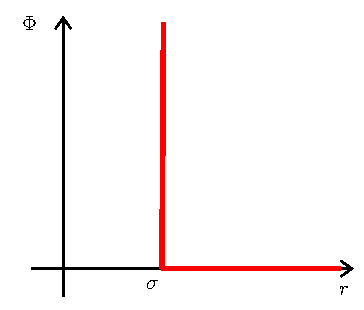
\includegraphics[width=0.5\textwidth]{./img/1__1.pdf}
\caption{\label{fig:15_12} Plot of the hard sphere potential \( \Phi (r) \).}
\end{figure}

In this case,
\begin{equation}
  f(\va{r}) = e^{-\beta \Phi (r)} -1 = \begin{cases}
    -1 & r < \sigma\\
    0 & r \ge \sigma
  \end{cases}
\end{equation}
Therefore, from the definition of \( B_2 \) and shifting to spherical coordinates:
\begin{equation*}
  B_2 (T)= - \frac{1}{2} \int_{V}^{} \dd[]{\va{r}}  f \qty(\abs{\va{r}} )
  = - \frac{1}{2} 4 \pi \int_{0}^{+ \infty } \dd[]{r} r^2 \qty[e^{-\beta \Phi (r)}-1 ]
  = 2 \pi \int_{0}^{\sigma } \dd[]{r} r^2 = \frac{2}{3} \pi  \sigma ^3
\end{equation*}
Hence,
\begin{equation}
  \Rightarrow B_2^{HS} (T) = \frac{2}{3} \pi  \sigma ^3
\end{equation}
this is the second virial coefficient for a hard sphere gas.
As expected \(  B_2^{HS} \) does not depend on temperature (purely repulsive interaction). Finally, for hard spheres we have:
\begin{equation}
  P V = N k_B T \qty(1 + \frac{2}{3} \pi \sigma ^3 \frac{N}{V})
\end{equation}
Note that the excluded volume interaction (hard sphere term) increases the product \( PV \) with respect to the ideal gas.

\subsubsection{Square wall potential}
We now use a slight refinement of the previous potential:
\begin{equation}
   \Phi ({\vec {r}})={\begin{cases}+\infty &|{\va {r}}|<r_{0}\\-\varepsilon &r_{0}<|{\va {r}}|<r_{0}+\delta \\0&|{\va {r}}|>r_{0}+\delta \end{cases}}
\end{equation}
This can be seen as a hard sphere potential where the spheres have an attractive shell of thickness \( \delta  \). We thus have:
\begin{equation}
f({\va {r}})={\begin{cases}-1&|{\va {r}}|<r_{0}\\e^{\beta \varepsilon }-1&r_{0}<|{\va {r}}|<r_{0}+\delta \\0&|{\va {r}}|>r_{0}+\delta \end{cases}}
\end{equation}
so that:
\begin{equation*}
\begin{split}
  B_{2} & =-{\frac {1}{2}}\int f(|{\va {r}}|)d{\va {r}}=-{\frac {1}{2}}\int 4\pi r^{2}f(r)dr=\\
  &=-2\pi \left[\int _{0}^{r_{0}}(-r^{2})dr+\int _{r_{0}}^{r_{0}+\delta }\left(e^{\beta \varepsilon }-1\right)r^{2}dr\right]=\\
  &=-2\pi \left\lbrace -{\frac {r_{0}^{3}}{3}}+{\frac {e^{\beta \varepsilon }-1}{3}}\left[(r_{0}+\delta )^{3}-r_{0}^{3}\right]\right\rbrace =B_{2}^{\text{h.s.}}-{\frac {2}{3}}\pi \left(e^{\beta \varepsilon }-1\right)\left[(r_{0}+\delta )^{3}-r_{0}^{3}\right]
\end{split}
\end{equation*}
where  \( B_2^{HS} \) is the first virial coefficient of the hard sphere potential we have previously seen. Now, if the temperature is sufficiently high, namely \(  \beta \varepsilon \ll 1\), we can approximate \( e^{\beta \varepsilon }-1\approx \beta \varepsilon \), so that:
\begin{equation}
  B_{2}=B_2^{HS} -{\frac {2}{3}}\pi \beta \varepsilon r_{0}^{3}\left[\left(1+{\frac {\delta }{r_{0}}}\right)^{3}-1\right]
\end{equation}
For the sake of simplicity, defining:
\begin{equation*}
  \lambda \equiv \left(1+{\frac {\delta }{r_{0}}}\right)^{3}-1
\end{equation*}
we will have, in the end:
\begin{equation}
  { \frac {PV}{Nk_{B}T}}=1+B_{2}\rho =1+\left(B_2^{HS} -{\frac {2}{3}}{\frac {\pi \varepsilon }{k_{B}T}}r_{0}^{3}\lambda \right)\rho
\end{equation}
so in this case  \( B_2 \) actually depends on the temperature.



\subsubsection{Lennard-Jones potential}
This potential is a quite realistic representation of the interatomic interactions. It is defined as:
\begin{equation}
  \Phi = 4 \varepsilon \qty[\qty(\frac{\sigma }{r})^{12} - \qty(\frac{\sigma }{r})^6  ]
\end{equation}
which contains a long-range attractive term (the one proportional to \( 1/r^6 \), which can be justified in terms of electric dipole fluctuations) and a short-range repulsive one (proportional to \( 1/r^{12} \), which comes from the overlap of the electron orbitals, i.e.Pauli excluded principle). This potential is plotted in Figure \ref{fig:15_13}.  The minimum is in \( r_{min}=2^{1/\sigma } \).   We can play with the range of attraction by changing \( \sigma  \) or by changing the   \( \varepsilon  \).


\begin{figure}[H]
\centering
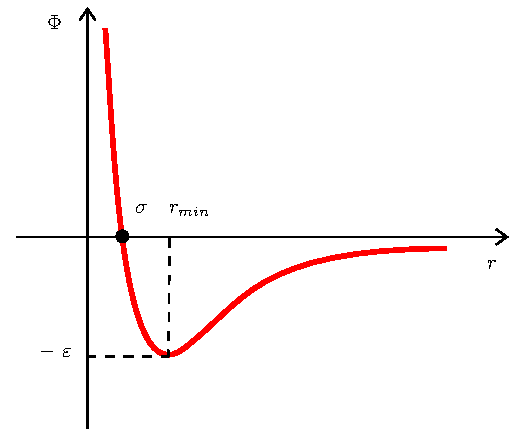
\includegraphics[width=0.5\textwidth]{./img/2__1.pdf}
\caption{\label{fig:15_13} Plot of the Lennard-Jones potential \( \Phi  \).}
\end{figure}
% What it is important is that for the Lennard-Jones we have
% \begin{equation}
%   B_2 \overset{LJ}{=} B_2 (T)
% \end{equation}

With this interaction potential, the first virial coefficient is:
\begin{equation*}
  B_2 (T) = - 2 \pi \int_{0}^{\infty } r^2 \qty[e^{- \frac{4 \varepsilon }{k_B T} \qty[\qty(\frac{\sigma }{r})^{12} - \qty(\frac{\sigma }{r})^6] } -1] \dd[]{r}
\end{equation*}
which is not analytically computable. However, it can be simplified defining the variables
\begin{equation*}
  x = \frac{r}{\sigma }, \qquad \tau = \frac{k_B T}{\varepsilon }
\end{equation*}
 so that, integrating by parts \( \int_{}^{} f' g = fg - \int_{}^{} g' f    \) where \( f' = x^2 g = \exp [-()]   \), we obtain
\begin{equation*}
\begin{split}
  B_2 (T^*) &= \frac{2}{3} \pi \sigma ^3 \frac{4}{\tau } \int_{0}^{\infty } x^2  \qty(\frac{12}{x^{12}}- \frac{6}{x^6}) e^{- \frac{4}{\tau } \qty(\frac{1}{x^{12}} - \frac{1}{x^6}) }  \dd[]{x}  \\
  & = A \int_{0}^{\infty } \qty(\frac{12}{x^{16}}- \frac{6}{x^4}) e^{- \frac{4}{\tau } \qty(\frac{1}{x^{12}} - \frac{1}{x^6}) } \dd[]{x}
\end{split}
\end{equation*}
Now, we can expand the exponential and integrate term by term; this gives an expression of \( B_2 \) as a power series of \( 1/\tau  \):
\begin{equation}
  B_2 (\tau ) = - 2 A' \sum_{n=0}^{\infty } \frac{1}{4n!} \Gamma \qty(\frac{2n-1}{4}) \qty(\frac{1}{\tau })^{\frac{2n+1}{4}}
\end{equation}
where \( \Gamma  \) is the Euler function and \( A' \) is a constant.  Note that the attractive part of the Lennard-Jones potential has introduced in \( B_2 \) a dependence on the temperature.





\subsection{Higher order terms in the cluster expansion}
Let us consider again the formal expansion
\begin{equation*}
  \prod_{i}^{} \qty(\prod_{j>i}^{} (1+f_{ij}) ) = 1 + \sum_{i,j>i}^{} f_{ij}
  + \sum_{\substack{ i \\ j>i \\ l>k \\ k \ge i \\ (ij) \neq (kl)} }^{} f_{ij} f_{kl}     + \dots
\end{equation*}
The problem with this expansion is that it groups terms quite different from one another. Fro example the terms \( f_{12}f_{23} \) and \( f_{12}f_{34} \). Indeed the first term correspond to a diagram as in Figure \ref{fig:15_1_1}, while the second to two disconnected diagrams as in Figure \ref{fig:15_1_2}.

\begin{figure}[H]
\begin{minipage}[c]{0.5\linewidth}
\subfloat[][Diagram of \( f_{12}f_{23} \). ]{ 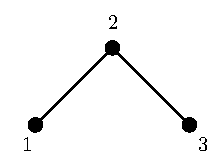
\includegraphics[width=0.6\textwidth]{./img/3__1.pdf}  \label{fig:15_1_1} }
\end{minipage}
\begin{minipage}[]{0.5\linewidth}
\centering
\subfloat[][Diagram of \(  f_{12}f_{34} \).]{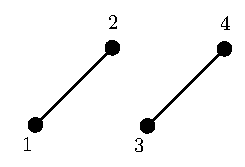
\includegraphics[width=0.6\textwidth]{./img/4__1.pdf}  \label{fig:15_1_2} }
\end{minipage}
\caption{\label{fig:} }
\end{figure} Another problem of the above expansion is that it does not recognize identical clusters formed by different particles. For example the terms \( f_{12} f_{23} \) and \( f_{12}f_{14} \) contribute in the same way to the partition function. It is then convenient to follow a diagrammatic approach similar to the Feymann approach in the reciprocal space.

\begin{minipage}[c]{0.7\linewidth}
For the linear term \( f_{ij} \) the only diagram is given by Figure \ref{fig:15_2}. As we have seen this has multeplicity
\begin{equation*}
\frac{N(N-1)}{2}
\end{equation*}
and the integral is of the form
\begin{equation*}
  \int_{}^{}  f_{12} \dd[]{\va{r}_1} \dd[]{\va{r}_2}  = V \int_{}^{} f(\va{r}) \dd[]{\va{r}}  = - 2 V B_2
\end{equation*}
\end{minipage}
\begin{minipage}[]{0.3\linewidth}
\centering
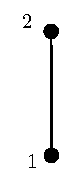
\includegraphics[width=0.3\textwidth]{./img/5__1.pdf}
\captionof{figure}{\label{fig:15_2} }
\end{minipage}

\vspace{0.5cm}
\begin{minipage}[c]{0.7\linewidth}
For the term \( f_{ij}f_{kl} \) we can have the case as in Figure \ref{fig:15_3},
that has molteplicity
\begin{equation*}
  \frac{N(N-1)}{2} \frac{(N-1)(N-3)}{2} \frac{1}{2}
\end{equation*}
 and the integral is of the  form
\begin{equation*}
  \int_{}^{}  f_{12} f_{34} \dd[]{\va{r}_1} \dd[]{\va{r}_2}  \dd[]{\va{r}_3}  \dd[]{\va{r}_4}
\end{equation*}
i.e. involving 4-particles
\begin{equation*}
\begin{split}
 &  \int_{}^{}  f( \abs{\va{r}_1 - \va{r}_2} )f( \abs{\va{r}_3 - \va{r}_4} ) \dd[]{\va{r}_1}  \dd[]{\va{r}_2}  \dd[]{\va{r}_3}  \dd[]{\va{r}_4}
  = \\
  & = V^2 \qty(\int_{}^{} f(\va{r})\dd[]{\va{r}}  )^2 = 4 V^2 B_2^2
\end{split}
\end{equation*}
\end{minipage}
\begin{minipage}[]{0.3\linewidth}
\centering
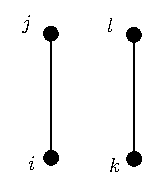
\includegraphics[width=0.6\textwidth]{./img/6__1.pdf}
\captionof{figure}{\label{fig:15_3} }
\end{minipage}

\vspace{0.5cm}

\begin{minipage}[c]{0.7\linewidth}
The next case if for instance as in Figure \ref{fig:15_4}. This involves 3 particles.
The multiplicity of this diagram is
\begin{equation*}
  \frac{N (N-1) (N-2)}{3!} \times 3
\end{equation*}
The integral is of the form
\begin{equation}
\begin{split}
  & \int_{}^{}  f_{12} f_{23} \dd[]{\va{r}_1}  \dd[]{\va{r}_2}   \dd[]{\va{r}_3}
  \simeq V  \qty(  \int_{}^{} \dd[]{r} f(r)  )^2  = \\
  & =   \int_{}^{}  f( \abs{\va{r}_1 - \va{r}_2} )f( \abs{\va{r}_2 - \va{r}_3} ) \dd[]{\va{r}_1}  \dd[]{\va{r}_2}  \dd[]{\va{r}_3}  = \\
  & = V \qty(\int_{}^{} f(\va{r})\dd[]{\va{r}}  )^2  = 4 V B_2^2
  \label{eq:15_3}
\end{split}
\end{equation}
\end{minipage}
\begin{minipage}[]{0.3\linewidth}
\centering
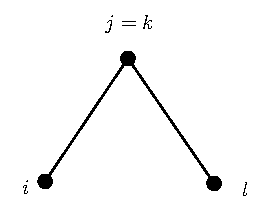
\includegraphics[width=0.8\textwidth]{./img/7__1.pdf}
\captionof{figure}{\label{fig:15_4} }
\end{minipage}

\vspace{0.5cm}

\begin{minipage}[c]{0.7\linewidth}
Another interesting diagram is the one in Figure \ref{fig:15_5}. Its molteplicity is
\begin{equation*}
  \frac{N(N-1)(N-2)}{3!}
\end{equation*}
The associated integral involves 3 particles and it is of the form
\begin{equation*}
\begin{split}
   & \int_{}^{} f_{12} f_{23} f_{31} \dd[]{\va{r}_1}  \dd[]{\va{r}_2} \dd[]{\va{r}_3} = \\
   & = \int_{}^{} f ( \abs{\va{r}_1 - \va{r}_2} ) f ( \abs{\va{r}_2 - \va{r}_3} )  f ( \abs{\va{r}_3 - \va{r}_1} )  \dd[]{\va{r}_1} \dd[]{\va{r}_2} \dd[]{\va{r}_3} \\
   & = \int_{}^{} f ( \abs{\va{r}_1 - \va{r}_2} ) f ( \abs{\va{r}_2 - \va{r}_3} )  f ( \abs{\va{r}_3 - \va{r}_1} )  \dd[]{\va{r}_2} \dd[]{\va{r}_{21}} \dd[]{\va{r}_{23}}
\end{split}
\end{equation*}
\end{minipage}
\begin{minipage}[]{0.3\linewidth}
\centering
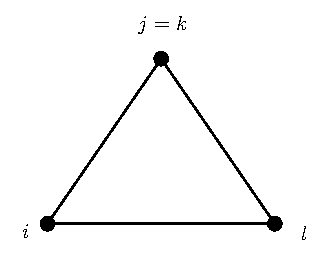
\includegraphics[width=0.8\textwidth]{./img/8__1.pdf}
\captionof{figure}{\label{fig:15_5} }
\end{minipage}

\noindent On the other hand \( \va{r}_{13} = \va{r}_{23} - \va{r}_{21} \), which implies
\begin{equation*}
   f ( \abs{\va{r}_3 - \va{r}_1} )  =  f ( \abs{\va{r}_{23} - \va{r}_{21}} )
\end{equation*}
Hence,
\begin{equation*}
  \int_{}^{} f (\abs{\va{r}_{12}} ) f (\abs{\va{r}_{23}} ) f (\abs{\va{r}_{31}} ) \dd[]{\va{r}_{21}}  \dd[]{\va{r}_{23}}  \dd[]{\va{r}_{2}}
   =  \int_{}^{} f (\abs{\va{r}_{12}} ) f (\abs{\va{r}_{23}} ) f (\abs{\va{r}_{23}-\va{r}_{21}} )  \dd[]{\va{r}_{21}}  \dd[]{\va{r}_{23}}  \dd[]{\va{r}_{2}}
\end{equation*}
Let us call this integral
\begin{equation}
  \int_{}^{} f_{12} f_{23} f_{31} \dd[]{\va{r}_1}  \dd[]{\va{r}_2}   \dd[]{\va{r}_3}
  \equiv  3! V  \qty( B_3 - 2 B_2^2  )
  \label{eq:15_4}
\end{equation}
The configurational partition function with the terms in Eq.\ref{eq:15_3} and Eq.\ref{eq:15_4} becomes
\begin{small}
\begin{equation}
\begin{split}
Q_N (V,T) = &  V^N - V^N \frac{N(N-1)}{V} B_2 + V^N\frac{ N (N-1)(N-2)(N-3)}{8V^2} (4B_2^2)
 + V^N \frac{N(N-1)(N-2)}{2V^2} 4B_2^2 \\
& = V^N \qty(1 + \frac{N(N-1)}{V} B_2 + \frac{N(N-1)(N-2)(N-3)}{2V^2} B_2^2 + \frac{N(N-1)(N-3)}{V^2} B_3)
\end{split}
\end{equation}
\end{small}

Let us now face the problem in a slightly different ways. Let us remind that
\begin{equation}
  Q_N (V,T) = \sum_{diagrams}^{} \int_{}^{} \prod_{kl}^{} f_{kl} \dd[3N]{r}
\end{equation}
where the sum is over all possible diagrams, i.e. all possible ways in which ones can draw edges between pairs of points \( (k,l) \).
For each such diagrams I have to product between all edge and then integrate over the configurational space (\( N \)  points).

 Let us now consider only \emph{connected} diagrams for \( i \) sites. In other words given \( i \) points (\( i \) particles)  from a system of \( N \) points and I consider all the possible ways I can connect these \( i  \) points (an example is shown in Figure \ref{fig:15_6}).
\begin{figure}[H]
   \centering
   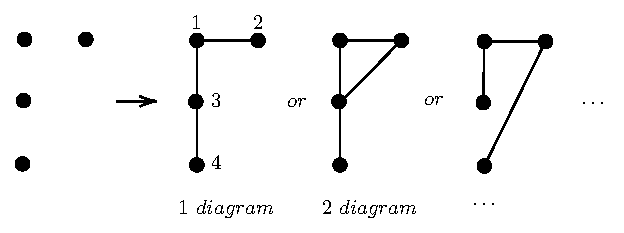
\includegraphics[width=0.7\textwidth]{./img/9__1.pdf}
   \caption{\label{fig:15_6} Example of connected diagrams for \( i=4 \) sites.}
   \end{figure}

For each diagram we take the product \( \prod_{kl}^{} f_{kl}   \) and then integrate over the position of the \( i \) points (\( i \) particles). For a fixed diagram:
\begin{equation*}
  \int_{}^{} \prod_{kl \in \, diagram }^{} f_{kl} \dd[]{\va{r}_1} \dots \dd[]{\va{r}_i}
\end{equation*}

\begin{example}{Diagram for \( \pmb{i=4} \) sites}{}
  For example the diagram 1 in Figure \ref{fig:15_6} gives the contribution
  \begin{equation*}
    \int_{}^{} f_{12} f_{13} f_{34} \dd[]{\va{r}_1}  \dd[]{\va{r}_2} \dd[]{\va{r}_3} \dd[]{\va{r}_4}
  \end{equation*}
  The diagram 2 gives
  \begin{equation*}
    \int_{}^{} f_{12} f_{13} f_{23} f_{34} \dd[]{\va{r}_1}  \dd[]{\va{r}_2} \dd[]{\va{r}_3} \dd[]{\va{r}_4}
  \end{equation*}
  and so on.
\end{example}

\noindent Finally, we sum over all these connected diagrams of \( i \) points:
\begin{equation*}
  \sum_{\substack{ \text{connected} \\  \text{diagrams} } }^{}    \int_{}^{} \prod_{lk \in \, diagram }^{} f_{kl} \dd[]{\va{r}_1} \dots \dd[]{\va{r}_i}
\end{equation*}
the results is what we call \( (i! V B_i) \) and defines \( B_i \). Let us analyze what happens for different values of \( i \) points:
\begin{itemize}
\item case \( i=1 \): clearly  \( B_1 =1 \);
\item case \( i=2 \): just one edge, hence we have just one connected diagram. The integral becomes:
\begin{equation*}
  \int_{}^{} f_{12} \dd[]{\va{r}_1} \dd[]{\va{r}_2} = - 2 V B_2
\end{equation*}
\item case \( i=3 \): the connected diagrams are shown in Figure \ref{fig:15_7}.
\begin{figure}[H]
\centering
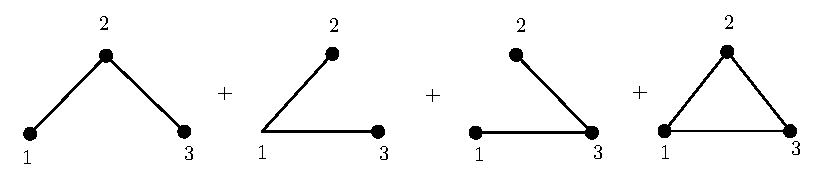
\includegraphics[width=0.8\textwidth]{./img/10__1.pdf}
\caption{\label{fig:15_7} Connected diagrams for \( i=3 \) points.}
\end{figure}

\begin{equation*}
\begin{split}
  & \sum_{\substack{ \text{connected diagrams } \\ \text{of \( i=3 \) points}} }^{} \int_{}^{} \prod_{kl \in \, diagram }^{} f_{kl} \dd[]{\va{r}_1}   \dd[]{\va{r}_2}    \dd[]{\va{r}_3} = \\
   &=  \underbrace{ \int_{}^{} f_{12} f_{23} \dd[]{\va{r}_1} \dd[]{\va{r}_2} \dd[]{\va{r}_3}
    + \int_{}^{} f_{12}f_{13} \dd[]{\va{r}_1} \dd[]{\va{r}_2} \dd[]{\va{r}_3}
    + \int_{}^{} f_{13}f_{23} \dd[]{\va{r}_1} \dd[]{\va{r}_2} \dd[]{\va{r}_3} }_{3 V \qty(\int_{}^{} f (\va{r})\dd[]{\va{r}}  )^2 }   \\
  & + \underbrace{\int_{}^{} f_{12} f_{23} f_{13} \dd[]{\va{r}_1} \dd[]{\va{r}_2} \dd[]{\va{r}_3}}_{3! V (B_3 - 2 B_2^2)}
\end{split}
\end{equation*}
Hence,
\begin{equation*}
\begin{split}
  \sum_{\substack{ \text{connected diagrams } \\ \text{of \( i=3 \) points}} }^{} \int_{}^{} \prod_{kl \in \, diagram }^{} f_{kl} \dd[]{\va{r}_1}   \dd[]{\va{r}_2}    \dd[]{\va{r}_3}
  & = 3 V (-2B_2)^2 + 6V (B_3 - 2 B_2) \\
  & = 6V B_3 = 3! V B_3
\end{split}
\end{equation*}

\end{itemize}

Eventually, for the partition function we have to sum over all possible clusters.
One possible procedure is:
\begin{enumerate}
\item given the \( N \) points we can partition them into connected clusters. For all \( i \) points we can make \( m_i \) clusters of that size \( i \).
\begin{equation*}
  \sum_{i}^{} i m_i = N
\end{equation*}
For each cluster of size \( i \) we have a term \( (i!VB_i) \). If there are \( m_i \) of them we have a weight \( (i! V B_i)^{m_i} \).
\item Now, we have to count in how many ways we can make the partition of \( N \) in a set of \( \{ m_i \}   \) clusters. Clearly if we permute the label of the \( N \) vertices we have possible different clusters. In principle, this degenerancy is proportional to \( N \)!

On the other hand, if one changes the order of the labels within a cluster (in \( i! \) ways) this does not change the cluster and since there are \( m_i \) clusters of size \( i \) we have to divide by \( (i!)^{m_i} \).

Moreover, since there are \( m_i \) clusters one can swap them (in \( m_i! \) ways). The degenerancy is \( \frac{N!}{m_i! (i!)^{m_i}} \). Therefore,
\begin{equation}
  Q_N (V,T) = \sum_{\{ m_i \}  }^{} \prod_{i}^{}    \frac{N!}{m_i! (i!)^{m_i}} \qty(i! V B_i)^{m_i}
\end{equation}
\end{enumerate}



\begin{figure}[H]
\begin{minipage}[c]{0.5\linewidth}
\subfloat[][Description]{ 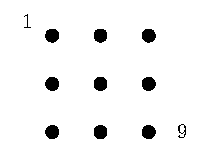
\includegraphics[width=0.8\textwidth]{./img/11__1.pdf}  \label{fig:15_8} }
\end{minipage}
\begin{minipage}[]{0.5\linewidth}
\centering
\subfloat[][Description]{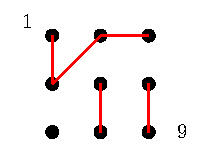
\includegraphics[width=0.8\textwidth]{./img/12__1.pdf}  \label{fig:15_9} }
\end{minipage}
\caption{\label{fig:} }
\end{figure}


\begin{exercise}{\( \pmb{N=9} \) points}{}
Consider the \( N=9 \) points in Figure \ref{fig:15_8}.
  \begin{enumerate}
  \item Partition these points into clusters, as in Figure \ref{fig:15_9}.

   For this partition \( \{ m_i \}   \) we have \( m_4=1,m_2=2,m_1=1 \). Now, the cluster of size 4 can be connected in a given different ways \( (4! V B_4)^1 \).
   \item Compute the degenerancy of this case (More on Huang chapter 10).
  \end{enumerate}
\end{exercise}





\end{document}
